\section*{\revise{Discussion}}
\label{sec:discussion}

That \ac{NSC} can explain and reproduce response properties observed in biological neurons may be an important clue as to how brains have evolved to parse and store information
\revise{in order to perceive the world and interact with it.
We offer two testable predictions of this theory:}
\mikeNote{I moved the Conclusions in here, because we seemed to repeat ourselves}

First, we predict that parts-based representations can explain
\acp{RF} of neurons in a variety of brain regions,
including but not limited to those brain areas discussed here. 
In agreement with the literature on basis function representations
\cite{PougetSejnowski1997,PougetSnyder2000,Poggio1990},
we expect parts-based representations
to be prevalent in regions where neurons
exhibit a range of tuning behaviors \cite{Beyeler2016},
display mixed selectivity \cite{Fusi2016,Eichenbaum2017},
or encode information in multiple reference frames \cite{AlexanderNitz2015,Rounds2016,Rounds2018}.

Second, where such representations occur, we expect the resulting
neuronal population activity to be relatively sparse,
in order to encode information both accurately and efficiently.
\revise{As noted above,}
sparse codes offer a trade-off between 
dense codes (where every neuron is involved in every context,
leading to great memory capacity but suffering from cross talk among neurons)
and local codes (where there is no interference, 
but also no capacity for generalization). %\cite{Spanne2015417}.
\revise{\ac{NSC} explicitly discourages statistically inefficient representations,
because strongly accounting for a rare observation at the expense of ignoring
more common input components would result in an increased reconstruction error
(see Eq.~\ref{eqn:nsc-cost-function}).}
\revise{Depending on input stimulus and task complexity,
we expect the level of sparsity in different brain areas to
be adjusted according to the bias-variance dilemma
(Fig.~\ref{fig:nsc-bias-variance-dilemma})}.

\revise{In summary, evidence reviewed in this paper suggests that
a variety of neuronal response properties can be understood
as an emergent property of efficient population coding 
based on dimensionality reduction and sparse coding.}



\subsection*{\revise{Potential neural mechanisms of NSC}}

\revise{As a special case of efficient coding,
\ac{NSC} possesses metabolic advantages by employing
sparse population codes.
To operate efficiently, it has been suggested that the brain might enforce 
geometrical and biophysical constraints on axonal wiring 
\cite{LaughlinSejnowski2003}.
In addition to reducing overall wiring length
\cite{Cherniak1994}, the brain might also aim to minimize local delays
by favoring a high degree of local connectivity
\cite{Chklovskii2002}.
With connectivity reflecting coding \cite{Clopath2010},
it would not be surprising to find that such ecological considerations
carry over into brain function,
favoring sparse population codes and neuronal representations that are
local in functional space (i.e., parts-based).
However, wiring cost is likely to be only one of many constraints 
on the brain connectome, perhaps supplementing competitive pressures
for hub-mediated information exchange between network modules
\cite{Rubinov2015}.}


% In addition, sparsity of the encoding might be enforced by spike thresholding \cite{Rozell2008} and lateral inhibitory connections \cite{Coultrip1992}.

\revise{In addition, evidence suggests that Hebbian-like synaptic plasticity rules
can perform statistical inference on their inputs
\cite{Nessler2009,Carlson2013,MorenoBoteDrugowitsch2015,Oja1982}.
One particular study demonstrated through a mathematical proof
that a certain form of \ac{STDP} in combination with 
homeostatic synaptic scaling (i.e., \ac{STDPH})
can approximate the \ac{NMF} algorithm
\cite{Carlson2013}.}
Similar to Oja's rule \cite{Oja1982}, which was developed to stabilize 
rate-based Hebbian learning
(effectively resulting in principal component analysis),
Carlson and colleagues showed that synaptic scaling acts as a 
homeostatic mechanism to stabilize \ac{STDP}
(effectively resulting in \ac{NMF}).
\revise{Interestingly, we were able to apply these ideas to 
electrophysiologically recorded neuronal activity observed in the \ac{RSC}
of rats during a spatial navigation task (Fig.~\ref{fig:NMF|RSC}; for experimental details see Supplementary Material). Both \ac{STDPH} and \ac{NMF} were able to recover key  features such as encoding spatial reference frames (i.e., allocentric, egocentric, and route-centric firing patterns) and position discrimination by reducing the dimensionality of behavioral variables (e.g., velocity, head direction, position).
The neuronal and population responses from NMF and STDPH were comparable to the experimental findings \cite{AlexanderNitz2015}.
\mikeNote{The way this section reads, I'm worried reviewers are going to say the figure should go in the Supplements, too. But, I didn't quite have the heart to do that.}
\jeffNote{I re-wrote this slightly.  I think the figure should stay. But, we need to be clear what these simulations show. It showed dimensionality reduction, but we can't make any claims on parts-based or sparsity}
Furthermore, the \ac{STDPH} model contained a highly flexible and generalizable code
that could automatically encode new routes through the same environment
without retraining \cite{Rounds2018}.
However, more research is needed to elucidate any potential connection 
between \ac{NSC} and the many different synaptic plasticity rules 
commonly found across brain regions,
different stages in the life of an animal, and animal species
(e.g., \cite{Froemke2010,BCM1982}).}


\begin{figure}[h]
	\centering
	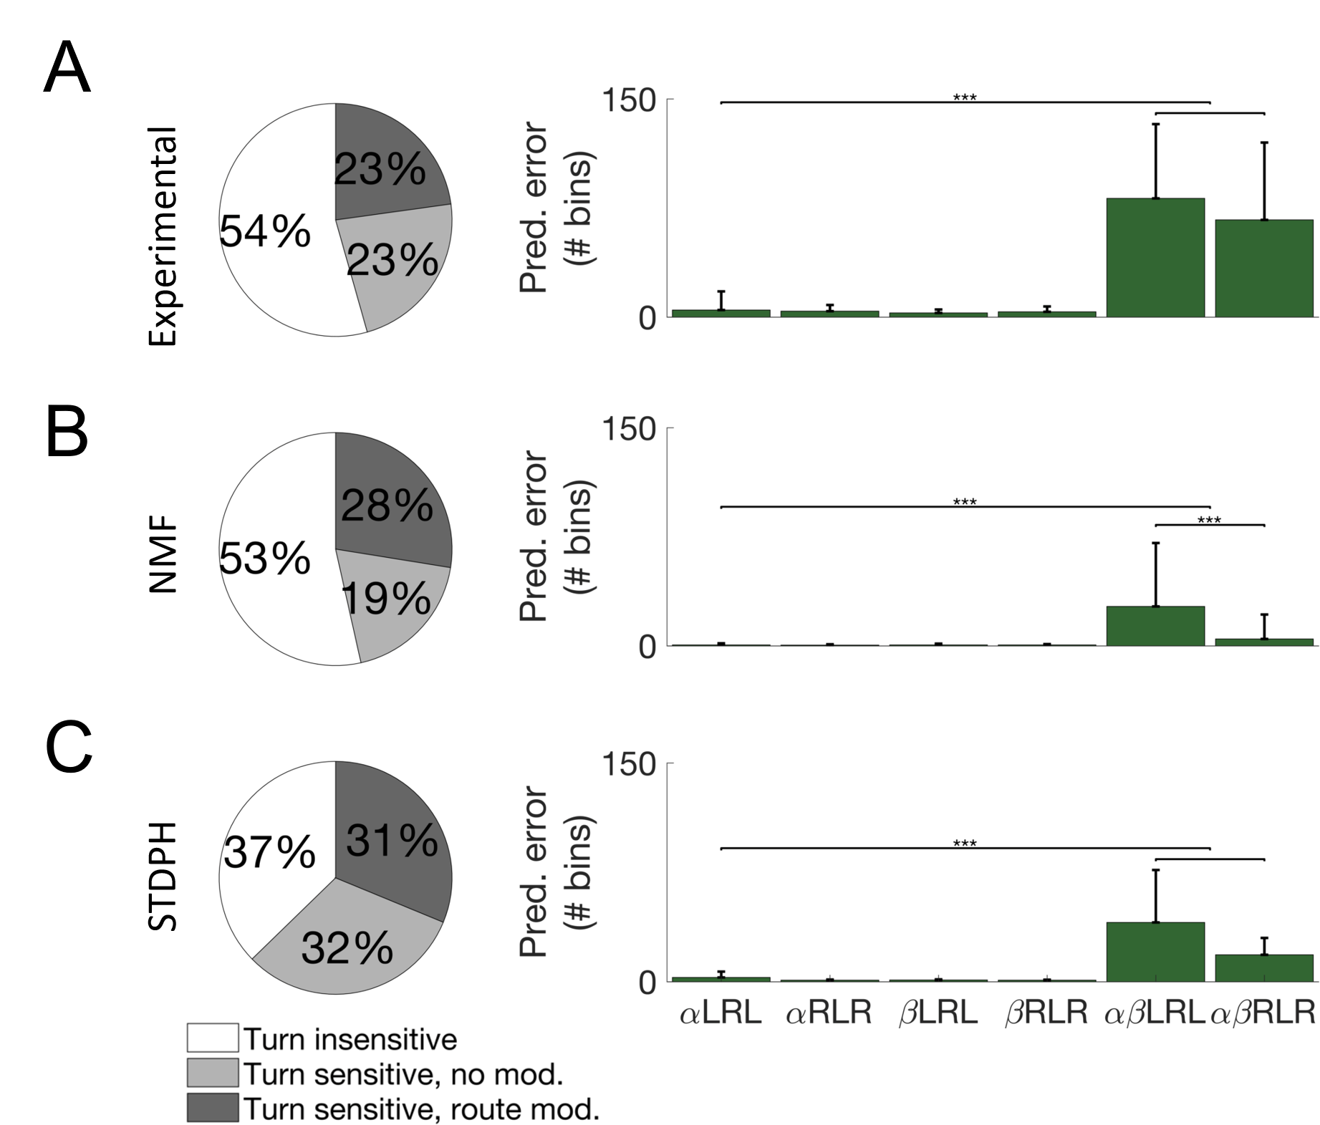
\includegraphics[width=\textwidth]{fig-rev1-rsc}
    \caption{\revise{Comparisons between recorded experimental data and two computational models of \ac{RSC} based on the data suggest a functional \revise{similarity} between \ac{STDPH} and \ac{NMF}. Using methods described in \cite{AlexanderNitz2015}, we compared functional neuron type distributions observed in experimentally recorded rat RSC neurons with the functional behavior of neuronal units}
         produced by each model (left columns) 
         and average error corresponding to \revise{correlation matrices representing reconstructed position within a route (right columns). For details, see Supplementary Materials.}
         Separate positions of the track are represented 
         by the symbols $\alpha$ and $\beta$. 
         Reconstructions between the track positions are represented by
         $\alpha$$\beta$.
      \textbf{\emph{A}},
         Experimental data from \cite{AlexanderNitz2015}.
      \textbf{\emph{B}},
         Simulated using NMF.
      \textbf{\emph{C}},
         Simulated by evolving STDPH parameters to fit experimental data.}
	\label{fig:NMF|RSC}
\end{figure} 



\subsection*{\revise{Model limitations}}

\revise{Although \ac{NSC} has proved useful in understanding
a variety of neuronal responses
as an emergent property of efficient population
coding based on dimensionality reduction and sparse coding,
there are some limitations to this theory.}

\revise{First, it remains to be demonstrated whether \ac{NSC} in its current form
can be extended to brain areas that require a dynamic process of information
gating, such as \ac{PFC} and motor cortex.
In these areas, diverse time courses across neurons have confounded
attempts to understand the basic encoding of decisions and movements.
However, the same is true for the olfactory system,
where population activity traces out loops that are organized by stimulus
condition. In particular, the orientation of the loop 
is related to the odor identity,
and the size of the loop is related to the odor concentration
\cite{Broome2006}.
Nevertheless, a recent \ac{NSC} based study was able to elucidate perceptually
relevant dimensions in odor space \cite{Castro2013}.
Our hope is that similar studies applied to \ac{PFC} and motor cortex will
reveal similar insights into their population response properties.}

\revise{Second, a practical limitation of dimensionality analyses in general
is that the apparent dimensionality of the population response changes
systematically with the complexity of the input stimulus
\cite{SpanneJorntell2015,Cowley2016,Mazzucato2016}.
For practical purposes, simulated models of neuronal circuitry are typically
built with far fewer units than the number of neurons in the real network.
By excluding input dimensions that are present in the brain,
one will implicitly guide the simulated model away from spurious interactions
that the real circuitry would have to handle.
As a result, the simulated model might underestimate 
the true complexity of the task.}

\revise{Third, the role of sparse coding in the brain has been questioned
\cite{SpanneJorntell2015}.
This is at least partly due to the wide variety of definitions of sparse
coding used in the literature:
In its widest possible theoretical sense,
a neuron population exhibits sparse activity if the average activation ratio
remains below 50\% in a binary neurons or below 100\% for thresholded,
rate-based neurons \cite{SpanneJorntell2015}.
However, it is not surprising that different brain areas might employ
different levels of sparsity.
Generalization requires that a population of neurons that supports a particular
input-output function must be able to accurately handle novel contexts.
The bias-variance dilemma (Fig.~\ref{fig:nsc-bias-variance-dilemma})
tells us that the level of complexity of the models represented in the brain
should be kept low because the resulting bias error of the models with
lower complexity is typicaly much smaller than the variance error of the
highly complex model.
Hence, the brain would ideally make do with a set of `good enough',
models, where the major advantages are that the capacity for generalization
increases.
This point of operation might differ drastically across brain areas---for example,
favoring an extremely sparse code in \ac{V1},
but giving rise to a slightly denser code with 
greater representational capacity in higher-order visual areas such as \ac{MSTd}, 
which could lead to compact and multifaceted encodings
of various perceptual variables
(see Discussion in \cite{Beyeler2016}).}
% \mikeNote{Integrate discussion section from: sparseness of mixed selectivity neurons controls generalization-discrimination trade off}
% % http://www.jneurosci.org/content/33/9/3844
\jeffNote{Is the bias-variance dilemma pertinent to the sparse coding challenge?  Does complexity relate to sparsity? I couldn't follow this argument.}


\subsection*{\revise{Model alternatives}}

\revise{Since \ac{NMF} is an integral part 
of Eq.~\ref{eqn:nsc-cost-function},
it is interesting to note that \ac{NSC} is tightly connected
to a number of unsupervised learning techniques,
such as $k$-means clustering,
an algorithm used to partition
$n$ observations into $k$ clusters
\cite{Ding2005}.
Due to its ability to decompose high-dimensional data into
sparse, interpretable factors, \ac{NMF} has become a 
widely used tool for the analysis of high-dimensional data,
with applications reaching far beyond
the field of computational biology
(for a recent review see \cite{Gillis2014}).}

\revise{In addition to the tight connection 
to linear sparse coding and \ac{NMF}
\cite{EggertKorner2004},
\ac{NSC} is also intimately related to \textbf{\ac{ICA}},
a computational method for separating a multivariate signal
into additive, statistically independent subcomponents. 
As originally noted by Hoyer \cite{Hoyer2002},
if the fixed-norm constraint is placed on the rows of
\textbf{H} instead of the columns of \textbf{W},
Eq.~\ref{eqn:nsc-cost-function} can be directly interpreted as the joint
log-posterior of the basis functions and hidden components
in the noisy \ac{ICA} model \cite{HoyerHyvarinen2002}.
In order for this connection to hold,
the \ac{ICA} basis functions must be chosen to be nonnegative,
and the independent components must have 
exponential distributions \cite{Hoyer2002}.}

\revise{Similarly, \ac{NSC} is closely related to compressed sensing
\cite{GanguliSompolinsky2012},
which posits that neurons might implement dimensionality reduction
by randomly projecting patterns of activity into a lower-dimensional space,
simply by synaptically mapping $N$ upstream neurons to a downstream region
containing $M < N$ neurons.
The theory of compressed sensing then provides the mathematical tools
to reconstruct the original space from the random projections.
\ac{NSC}, \ac{ICA}, and compressed sensing often make similar predictions
that only slightly differ in the nature of the basis function representation
necessary to achieve optimal reconstruction
(for details please refer to the Discussion of \cite{GanguliSompolinsky2012}).
For example, whereas \ac{ICA} emphasizes the statistical independence 
of unmixed sources
and compressed sensing requires basis function to be `maximally incoherent'
\cite{GanguliSompolinsky2012},
\ac{NSC} does not make any such assumptions
as long as the basis functions are nonnegative.}




% Furthermore, NSC has implications for computing, artificial intelligence, and machine learning. \ac{NSC} can be used to design neural networks that are highly compressed, so that the number of neurons is far smaller than the number of input features represented. 
% Moreover, these networks can represent data with a sparse code,
% % \mikeNote{No need to explain sparse coding again}
% % ; that is, when input data is presented to the network, only a few neurons are active at any given time,
% making the code very energy-efficient.
% At the same time, different data samples might activate a different subset of neurons, making the code highly informative. By taking linear combinations of neural activity (i.e., linear decoding), the system can infer latent variables that are unobservable in the original high-dimensional dataset \cite{PougetSnyder2000}.





